\scanpage{5}

\margin{\figure{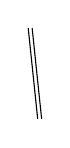
\begin{tikzpicture}\draw (0,0)--(-.12,1.15);\draw (.05,0)--(-.07,1.15);\end{tikzpicture}}}
sont \unsure{duals|duaux} l'un de l'autre, et que
\[
H^p(A,\Omega_A^q)\text{ est dual de }H^q(B,\Omega_{\unsure{A}}^p).
\]

[Ce dernier fait, grâce à :
\[
H^*(A,\Omega_A^*)=\bigwedge\bigl(H^*(A,\Omega_A^*)\bigr)^{(1)}
\]
se ramène au cas de la \unsure{dim} $1$, i.e. par symétrie à la dualité de $H^1(A,\uline{O}_A)$ et $H^0(B,\uline{\Omega}_B^1)$, qui est immédiate. \deleted{De plus,} \unsure{or}, pour avoir une dualité entre $H^*(A)$ et $H^*(B)$, il \unsure{suffirait} grâce à la structure connue de la définir entre $H^1(A)$ et $H^1(B)$, ce qui ne saurait offrir de difficultés....

Il y a lieu enfin de comparer ces extensions et dualités avec ce que donne la \uline{dualité de Cartier}. \unsure{Considérons} (la car. étant : $p>0$) $\unsure{p^A|{}_p A}$ qui est dual au sens Cartier de $p^B$. On a aussi $F^A=\operatorname{Gr}(t_A)\subset p^A$ ; de degrés respectifs $p^{\deleted{\unsure{2}}d}$ et $p^{2d}$, où $d=\dim A$.
\diagram{\begin{array}{l}
F^A\subset p^A\\[1ex]
F^B\subset p^B
\end{array}\Biggr]\ \text{\unsure{duals|duaux} l'un de l'autre}}
Je dis que $F^A$ \uline{et} $F^B$ \uline{sont orthogonaux l'un de l'autre}. \deleted{\unsure{Notons que} $F^B$} On le

\mspage{4}
